\chapter{Porovnání s existujícími nástroji}

\section{Jak probíhalo testování?}
Testování probíhalo na vzorové stránce, která byla připojena k databázi s katalogem hudby (viz kapitola 3). Testovací stránka obsahovala 4 formuláře různých typů a odkazy. Polovina parametrů byla nezabezpečených, tudíž mohli být napadnuty.

\section{OWASP ZAP}
\subsection{Co je OWASP ZAP?}
\textit{The Open Web Application Security Project} je celosvětová nezisková charitativní organizace\cite{owasp}, jejíž cílem je zvýšit zabezpečení softwarových řešení. Veškeré jejich snahy jsou cíleny na zviditelnění možností bezpečnostních opatření. Všechny materiály, knihy a software, který je vyvíjen je zdarma. 

\begin{figure}[h!]
\centerline{
\includegraphics[width=325px]{./examples/owasp.jpeg}}
\caption{https://www.owasp.org/}
\label{owasp}
\end{figure}

\subsection{OWASP ZAP}
\textit{OWASP Zed Attack Proxy Project} je penetrační test pro nalezení bezpečnostních chyb ve webových aplikacích, umožňuje manuální kontrolu i automatické testy. Je k dispozici zdarma na: \textit{https://code.google.com/p/zaproxy/}.

\subsection{Nalezené výsledky}
OWASP na testovací stránce nezjistil vůbec žádné problémy typu SQL injection, i když byly zapnuty chybové direktivy. Detekoval ovšem dalších mnoho problémů s procházením adresářů či špatném zasílání hlaviček.

\section{SQLMap}
\textit{SQLMap - Automatic SQL Injection and database takeover tool}, tato utilita byla zajímavější než výše předchozí OWASP. Je napsána v jazyce Python a je zdarma k dispozici na \textit{http://sqlmap.org/}. Dokáže přes nezabezpečený parametr získat veškeré informace o databázovém serveru, vytvořit uživatele (je-li to možné) nebo získat struktury tabulek celé databáze.

\subsection{Nalezené výsledky}
Nepodařilo se mi realizovat, aby SQLMap stránky prohledával sám (jako to dělá OWASP), ale při nalezení nezabezpečeného vstupu se ukázal jako výborný pomocník (jak už název napovídá) k převzetí databáze, což se na nezabezpečeném vstupu povedlo bez problémů.

\section{OWASP / SID + SQLMap}
SQLMap a OWASP / SID dohromady tvoří zajímavý nástroj pro detekci a následné \uv{zneužití} SQL injection chyby. OWASP by byl využit pro zjištění všech možných vstupů, které by následně SQL Map otestoval, které je značné množství a SQL Map provádí testy opravdu dlouho. Při využití SIDu a SQL Mapu bude tento čas menší. Při testech SID + SQL Map na vlastním serveru jsem získal všechny tabulky a data z nich.

\section{Acunetix - Web Vulnerability Scanner}
Tento nástroj nebyl v testu použit, protože je placený a není k dispozici pro jiné operační systémy než je Microsoft Windows. Dle informací od výrobce (\textit{http://www.acunetix.com/}) by měl být schopen automaticky detekovat jak SQL Injection tak XSS problémy.


\chapter{Ukázky použití SID}
\subsection{Stažení a instalace}
SID je možné se zdrojovými kódy stáhnout z GIT repozitáře, který je umístěn na serveru GitHub, kde byl v rámci bakalářské práce vyvíjen. Repozitář je read-only, takže je možné ho standardní cestou naklonovat. Dále je přiložen soubor \textit{Gemfile} a \textit{Rakefile}. První ze souborů umožňuje automatické stažení potřebných balíčků (tzv. \textit{Gemů}) pro spuštění programu. Druhý (\textit{Rakefile}) slouží pro automatické spuštění testů ze složky \textit{test}. Celý postup je uveden v následující části \ref{SID_instalace}.
\begin{lstlisting}[label=SID_instalace,language=Bash, caption=Instalace]
# Klonovani repozitare
git clone git@github.com:Strnadj/SID.git SID

# Presun do slozky penetracniho testu
cd SID/PenTest

# Stazeni potrebnych balicku
bundle

# Spusteni vsech testu - volitelna moznost
rake

# Presun do slozky se spustitelnou binarkou
cd bin/

# Spusteni testu
./pentest 

\end{lstlisting}
Pokud vše proběhlo správně, zobrazí se nápověda v příkazové řádce s možnými parametry. Jediný povinný parametr je \textit{-u}, kterým zadáváme URL, která se bude zpracovávat. Ostatní parametry jsou nepovinné.

\subsection{Ukázka spuštění}
Pro základní spuštění použijeme následující příkaz:
\begin{lstlisting}[label=SID_run,language=Ruby, caption=Spuštění testu]
./pentest -u http://localhost/test/ -d true -e false
\end{lstlisting}
Používáme tři parametry:
\begin{enumerate}
\item \textit{-u} - URL testované stránky
\item \textit{-d} - tzv. \textit{debug/verbose} mód, který vypisuje veškeré informace o probíhajícím testu
\item \textit{-e} - nastavení zobrazování chyb na serveru, pokud uvedeme false tak jsou direktivy vypnuté a porovnává se obsah
\end{enumerate}
Pokud test spustíme bez parametrů zobrazí se nápověda se seznamem parametrů, které můžeme použít a jejich popisem.

\subsection{Identifikace podezřelé proměnné}
Pokud test nalezne proměnnou, která je podezřelá na SQL injection, je přehledně vypsána i s testovacími URL, které byly použity. Administrátor následně může tyto URL zkontrolovat a zkontrolovat parametry (pro identifikaci ve zdrojových kódech můžeme využít například příkaz  grep).
\begin{figure}[h!]
\centerline{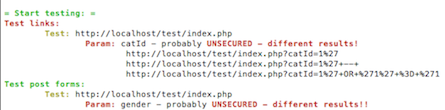
\includegraphics[]{./examples/SID-succ2.png}}
\caption{Úspěšné nalezení nezabezpečeného parametru}
\label{chart.attack}
\end{figure}